\subsection{Implementation details}

The following will go over some specific details of the code implementation.
An explanation as to why a new MD code was written is first presented. The
model approximating the cluster environment for atomic processes is then
presented, followed by specific details to photon and impact ionization.
Next, the use of cross-sections for ionization events is explained and finally
recombination as implemented in the code is presented.


\subsubsection{MD code}

Our group previously used Barnes and Hut's treecode implementation,
freely available\cite{treecode} (through the GPL version 2 license). The code was adapted
to simulate charged particles (Coulomb force) instead of masses (gravitational
force) with some ionization routines added (see for example reference
\cite{Jungreuthmayer2005}). While reducing development time by re-using already
written code, the maintenance burden introduced by many factors (initial
implementation written in the C language, usage of global variables
throughout the code, multiple coding styles from different people throughout
the years, lack of revision control system giving freedom
of deleting code from the active version without losing the ability to roll
back, many subtle and important bugs, stability issues, etc.) convinced me
to start from scratch. This allowed modern development techniques to be
used. For example, all development was done through a revision control system
(subversion\cite{svn} at first, then switched to git\cite{git}) in the C++
language instead of C. The object oriented nature of C++ allowed encapsulation
of different parts of the code which could then be tested and validated
individually through unit testing. This gave much better flexibility to the
code, a required asset to
push further the development of features.

A substantial number of MD packages are freely available and
their use was considered instead of re-implementing a new one from scratch.
Examples are GROMACS\footnote{GROMACS:
\url{http://www.gromacs.org/}}, NAMD\footnote{NAMD:
\url{http://www.ks.uiuc.edu/Research/namd/}} and
LAMMPS\footnote{LAMMPS: \url{http://lammps.sandia.gov/}}. A major issue with these
pre-existing MD packages is their target audience; they aim to simulate large
bio-molecules with mostly short range interactions. Another important problem
is the number of particles throughout the simulations. While many packages
assume a constant number of particles, the present work required creating
(ionization) and annihilating (recombination) particles during simulations.
Controlling the MD part of the code allowed better integration of the
ionization aspects.

Additionally, other MD packages were not mature enough or simply non-existent at the time.
For example the largely used HOOMD-blue\footnote{HOOMD-blue:
\url{http://codeblue.umich.edu/hoomd-blue/}} which uses extensively
Nvidia GPUs released its first version (v0.6.0) in February 2008.
The knowledge and experience gained by writing from scratch such
a package is also invaluable.




\subsubsection{Potential threshold $V_b$}
\label{section:intro:Vb}

Many ionization processes described in the introduction
consider an isolated atom but
clusters have close to solid density (10$^{22}$ -- 10$^{23}$ cm$^{-3}$);
the cluster environment cannot be ignored.

This environment can be approximated by a constant value that shifts the
potential\cite{Fennel2007}. The shift is $U_b = -e_0 V_b$ where $V_b$ is the
potential due to the cluster at the ion's location (ignoring nearby electrons)
and $U_b$ is the potential energy a test particle of charge state -1 (an electron)
would have if it were placed right on top of the ion. This can be justified by
the fact that bound states of rare gas atoms are localized close to the nucleus
and the cluster potential spatial variation around atoms is small.

To illustrate this shifting, figure \ref{fig:md:Vb} shows the potential energy
landscape of an example ``cluster'' of two ions. Plotted on this figure is the
potential energy of a test particle of charge state -1 (an electron) in the
cluster environment. The contribution from the ion is the blue dashed line on the
figure. Note the distinction between potential and potential
energy. A positive charge (an ion) creates a positive potential but the
potential \textit{energy} of the test particle (of charge state -1) in that
positive potential is negative, hence the negative curves on figure
\ref{fig:md:Vb}.



\begin{figure}
    % ./potential_landscape.py --two --ion="0,1" --ion="-15,5" --impe_r=4 \
    %     --depth=1.5 --ion_impe=0 --impe_K=0.75 --ionization --umin=-1.2 \
    %     --umax=0.3 --plot=all --rmin=-7 --rmax=7.5 --plot=U
    \begin{center}
    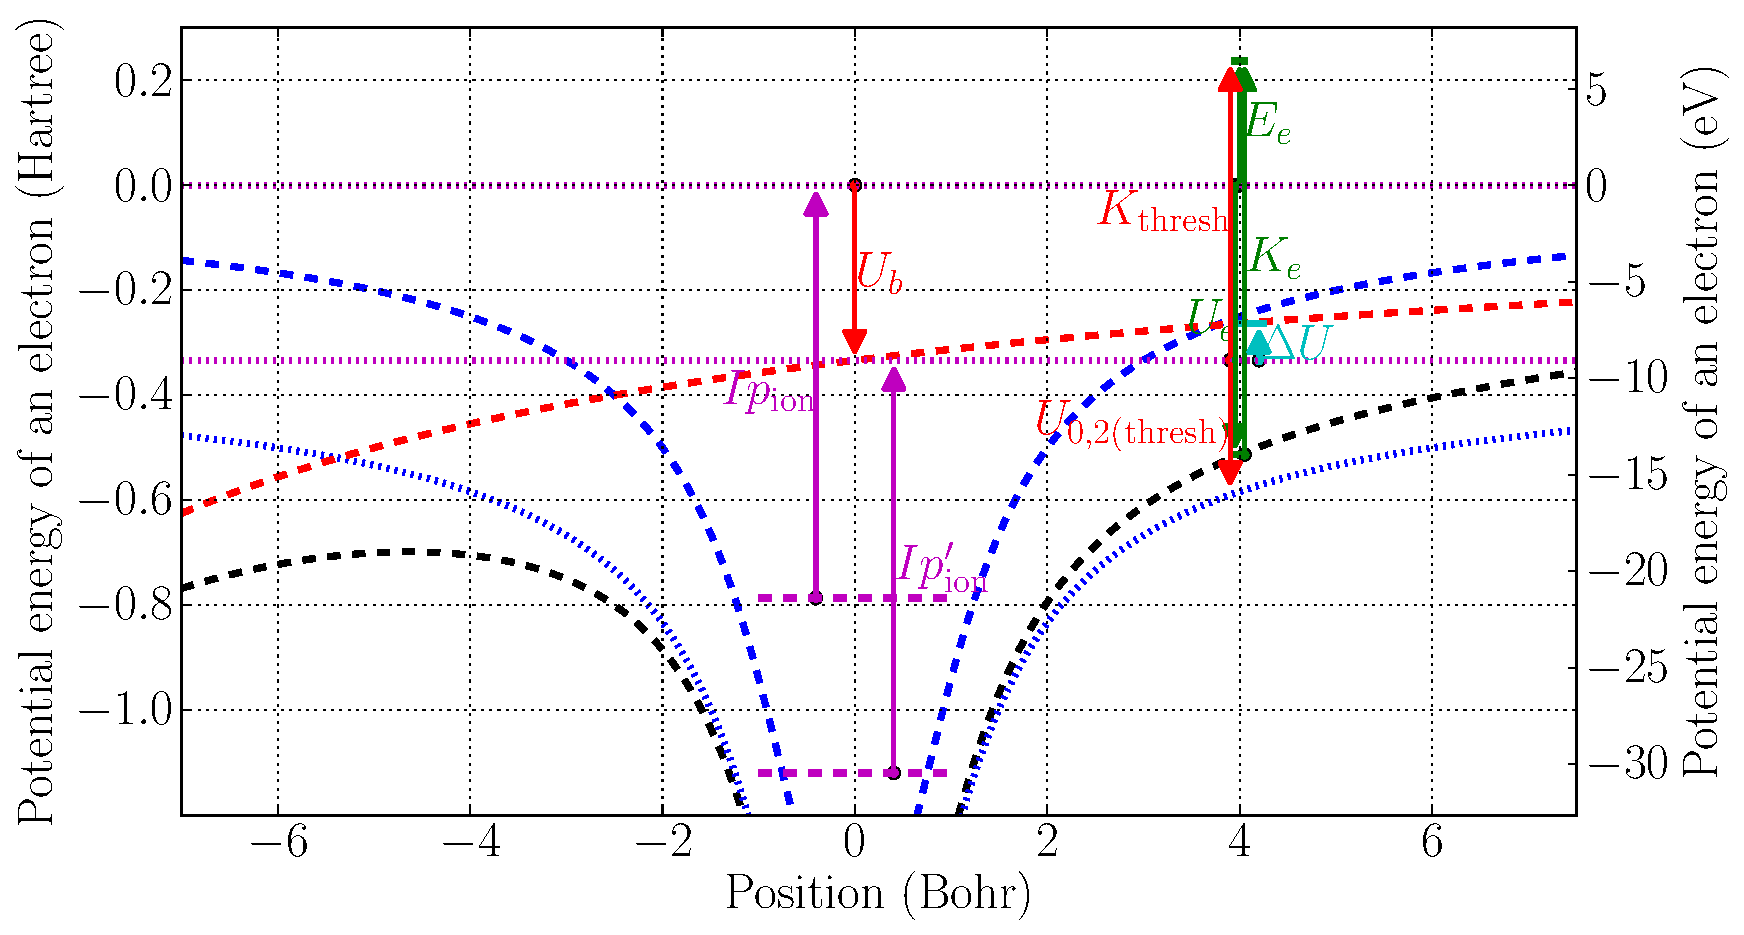
\includegraphics[width=\figurewidth]{figures/potential_landscape}
    \end{center}
    \caption{\label{fig:md:Vb}Cluster environment potential energy landscape
             and the $U_b$ approximation. A 1+ ion at $r=0$ and a 5+ at
             $r=-15$~Bohr. The potential energy curves are those of a test
             particle of charge state -1 (electron).
             The first ion's contribution is in blue-dashed line. The second ion's
             contribution is in red-dashed line and represents the cluster environment.
             The black-dashed line represents the total from the two ions.
             The blue-dotted line is the first ion's potential shifted by $U_b$.
             The upper horizontal magenta-dotted line is the isolated atom
             threshold, while the lower one is the shifted one due to the cluster
             environment.}
\end{figure}


Continuing in the example case of figure \ref{fig:md:Vb}, we introduce a
second ion as an example of the simplest cluster environment. This second ion, of
charge state 5+ in this example and located at $r$~=~-15 Bohr, is creating a
potential that is not constant around the first ion (red-dashed line). The potential energy of
the test particle in this potential is plotted as the red dashed line. The total
potential energy of the test particle due to the two ions is plotted as a black
dashed line.

The first ion's threshold is thus influenced by the second ion. The continuum,
instead of being at zero, is shifted by $U_b$. This approximates the
influence of the second ion as being constant in the first ion's vicinity. This
threshold shift is shown on figure \ref{fig:md:Vb} as the red arrow $U_b$.

The effect of $U_b$ is to shift the ion's states to lower energies. This is
shown on the figure as Ip$_{ion}$, the energy required for a bound electron
to be promoted to the isolated ion's continuum, being shifted downward to
Ip$_{ion}'$. The effective ion's potential energy curve, also shifted by $U_b$,
is shown as the dotted blue line.

This cluster potential $U_b$ is then treated as the atom's threshold
to continuum. By using $U_b$ as the threshold, atomic properties such as
impact ionization cross-sections can be used, even in the cluster environment.



\subsubsection{Notes on ionization definition}
\label{section:intro:mechanisms:notes}

Special care needs to be taken when calculating particle energies during
ionization processes. In this work, an ionization event is defined as one
electron that leaves its isolated parent ion, reaching infinity with a final
kinetic energy of zero.

As described in the previous chapter \ref{section:intro:Vb} (page
\pageref{section:intro:Vb}), the cluster
influence on ionization is approximated as a new threshold, which we call $V_b$.

The following paragraphs will discuss some specific details concerning single
photon ionization and impact ionization, both in the special case of an isolated
atom or ion. The generalization to the cluster environment is done through the
updated threshold, as discussed in chapter \ref{section:intro:Vb} (page
\pageref{section:intro:Vb}).


\subsubsubsection{Single photon ionization}

In the case of single photon ionization, a new electron is created right on top
of the ion with an updated charge state. At this point, all other particles in
the cluster will not see a difference; the potential $\phi'\pa{\vr}$ created by
this new particles pair
\begin{align}
\phi'\pa{\vr} & = \phi_{j}\pa{\vr;Z+1} + \phi_{k}\pa{\vr;-1},
\end{align}
is the same as the previous ion's $\phi_{j}\pa{\vr;Z}$ (see equation
\eqref{eqn:md:smoothed:phi} for the potential shape mainly used).


For the new electron to reach infinity with a null kinetic energy, it
must have, at its creation time, enough kinetic energy to leave the ion. This
kinetic energy must thus match the potential energy between the ion (with an
updated charge state) and the electron so the total energy of the electron with
respect to the ion is zero.

Additionally, the electron will contain in its kinetic energy the difference
between the absorbed photon and the ionization potential of the ion.


\subsubsubsection{Impact ionization}

For impact ionization (still in the case of an isolated atom),
the impacting electron's kinetic energy used in equation
\eqref{eqn:impact:ionization:lotz} is the kinetic energy the electron has
\textit{at infinity}, meaning that the impacting electron and the isolated
atom (or ion) are separated in an unbound system.

At infinity, the electron's total energy only contains kinetic
energy. We call this kinetic energy $K_{\textrm{thresh}}$ for ``kinetic energy
above the threshold''. This $K_{\textrm{thresh}}$ can simply be calculated
as $K_{\textrm{thresh}} = \textrm{max}\pa{0, K_e + U_e}$
where $K_e$ is the
electron's kinetic energy and $U_e$ its potential energy with respect to the ion.
$K_{\textrm{thresh}}$ is thus the electron's total energy \textit{with respect
to the ion}.
In the case of a classically bound electron, the total energy is less than zero:
the max() enforces a positive kinetic energy.

When a cluster environment is present, a similar approach is taken to obtain
$K_{\textrm{thresh}}$. Instead of taking the extra energy above zero for
$K_{\textrm{thresh}}$, the extra energy above the new threshold $U_b$ is used.
This value can easily be obtained from the actual electron's kinetic energy
$K_e$, it's \textit{total} potential energy in the cluster environment and the
threshold $U_b$ by:
\begin{align}
K_{\textrm{thresh}} & = \textrm{max}\pa{0, K_e + U_e - U_b}
\label{eqn:md:kthresh}
\end{align}
and is shown on figure \ref{fig:md:Vb} as a red arrow with its base at $U_b$.


$K_{\textrm{thresh}}$ is the kinetic energy that must be used in Lotz formula
\eqref{eqn:impact:ionization:lotz}. Cross-sections are discussed in the next
section.


When an impact ionization event occurs and if the impacting electron has more kinetic
energy, it can either keep the extra, give all the extra, or give a fraction of
the extra to the new electron. We split the extra kinetic energy between the two
electrons to assure that they do not fall back into the ion.


% Figure \ref{fig:impact:before:Z} shows the process of impact ionization when an
% electron (particle 1) of charge state -1 impacts an ion (particle 0) of charge
% state Z and creates a new electron (particle 2) right on top.
%
% \begin{figure}
%  \centering
%     \begin{subfigure}{0.48\columnwidth}
%         \centering
%         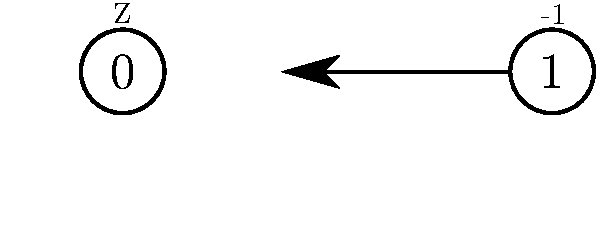
\includegraphics[width=\textwidth]{figures/impact_ionization_t00}
%         \caption{Before impact ionization (Z)}
%         \label{fig:impact:before:Z}
%     \end{subfigure}
% \\
%     \begin{subfigure}{0.48\columnwidth}
%         \centering
%         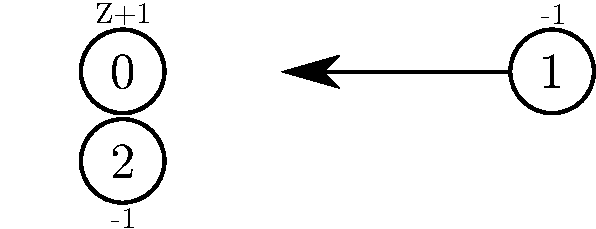
\includegraphics[width=\textwidth]{figures/impact_ionization_t0}
%         \caption{During impact ionization (Z+1)}
%         \label{fig:impact:before:Zp1}
%     \end{subfigure}
% %
%     \begin{subfigure}{0.48\columnwidth}
%         \centering
%         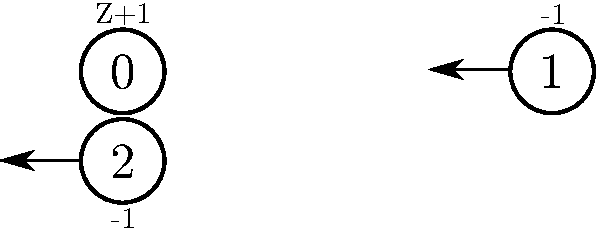
\includegraphics[width=\textwidth]{figures/impact_ionization_t1}
%         \caption{After impact ionization}
%         \label{fig:impact:after}
%     \end{subfigure}
% \caption{Impact ionization: before and after}
% \label{fig:impact:steps}
% \end{figure}


% First, let's assume the impacting electron came from infinity where it's kinetic
% energy was exactly the Ip. In that case, impact ionization will occur (considering
% its impact parameter lies inside the cross-section). By definition, we must have two
% electrons leaving to infinity: an unbound system. Such an unbound system has a total
% energy of 0.
%
% The total energy before (a) is thus:
% \begin{align}
% E^{a} & = K_{1}^{a} + U_{01}^{a} = Ip
% \label{eqn:Ea}
% \end{align}
% and after (c) ionization is:
% \begin{align}
% E^{c} & = K_{1}^{c} + K_{2}^{c} + U_{01}^{c} + U_{02}^{c} + U_{12}^{c} = 0
% \label{eqn:Ec}
% \end{align}
%
% The change in energy is thus:
% \begin{align}
% E^{a} - E^{c} & = Ip = K_{1}^{a} + U_{01}^{a} - \pa{
%     K_{1}^{c} + K_{2}^{c} + U_{01}^{c} + U_{02}^{c} + U_{12}^{c}
% }
% \end{align}
%
% The only unknown values here are $K_{1}^{c}$ and $K_{2}^{c}$ since the new electron is
% created right on top of the ion. Let's isolate the final kinetic energies:
% \begin{align}
% K_{1}^{c} + K_{2}^{c} = K_{1}^{a} + U_{01}^{a} - \pa{
%     U_{01}^{c} + U_{02}^{c} + U_{12}^{c}
% } - Ip
% \label{eqn:K1cPlusK2c}
% \end{align}
%
% We have a single constraint from equation \eqref{eqn:K1cPlusK2c} but two unknown. We thus
% give an arbitrary value to one of the two. We want the new electron to leave the ion.
% Since it is right on top of it, we can guess the required kinetic energy to be very close
% to (minus) the potential energy the electron has with respect to the ion. But this electron
% will be ``pushed'' be the impacting electron too and will thus be accelerated. To compensate
% for this push, we remove the potential energy between the two electrons from the new electron's
% kinetic energy. So the educated guess for the final kinetic energy of the new electron is:
% \begin{align}
% K_{2}^{c} & = -U_{02}^{c} - U_{12}^{c}
% \label{eqn:K2c:pushed}
% \end{align}
%
% Using equation \eqref{eqn:K2c:pushed} in equation \eqref{eqn:K1cPlusK2c} gives:
% \begin{align}
% K_{1}^{c}
%  & = K_{1}^{a} + U_{01}^{a} - \pa{
%     U_{01}^{c} + U_{02}^{c} + U_{12}^{c}
% } - Ip - K_{2}^{c} \\
%  & = K_{1}^{a} + U_{01}^{a} - \pa{
%     U_{01}^{c} + \cancel{ U_{02}^{c} } + \bcancel{ U_{12}^{c} }
% } - Ip + \cancel{ U_{02}^{c} } + \bcancel{ U_{12}^{c} } \\
% K_{1}^{c}
%  & = K_{1}^{a} + U_{01}^{a} - U_{01}^{c} - Ip
% \label{eqn:K1c:pushed}
% \end{align}
%
% The final total energy is then:
% \begin{align}
% E^{c}
%  & = \pa{
%     K_{1}^{a} + U_{01}^{a} - \cancel{ U_{01}^{c} } - Ip
%  } - \pa{
%                  \cancel{ U_{02}^{c} } + \bcancel{ U_{12}^{c} }
% } + \cancel{ U_{01}^{c} } + \cancel{ U_{02}^{c} } + \bcancel{ U_{12}^{c} } \\
%  & = K_{1}^{a} + U_{01}^{a} - Ip \\
%  & = Ip - Ip \\
% E^{c} & = 0
% \end{align}
% which is what was expected.






% Additionally, momentum is conserved by giving the two leaving electrons an angle
% of divergence. Since the impacting electron can cause ionization before being
% exactly on top of the atom or ion, the angle of divergence is given by:
%
% Figure \ref{fig:impact:direction} shows the convention of the two angles $\theta$ and $\phi$.
%
% \begin{figure}
% \begin{center}
% 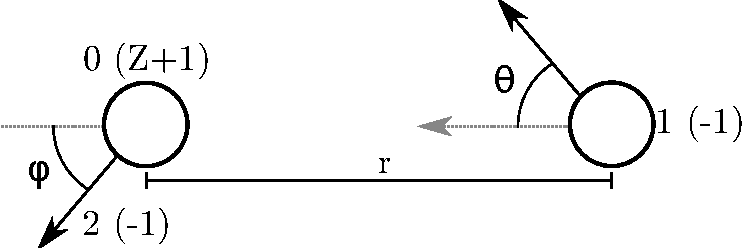
\includegraphics[width=0.8\textwidth]{figures/impact_ionization_directions}
% \end{center}
% \caption{Impact ionization: Direction for electrons}
% \label{fig:impact:direction}
% \end{figure}
%
%
% Momentum is conserved in each dimension. In this case, it's a 2-D plane.
% \begin{align}
% \vp^{a} & = \vp^{c} \\
% \vp^{a} & = m_e v_{1x}^{a} \hat{x} \\
% \vp^{c} & = m_e \pa{v_{1x}^{c} + v_{2x}^{c}} \hat{x} + m_e \pa{v_{1y}^{c} + v_{2y}^{c}} \hat{y}
% \end{align}
% with:
% \begin{subequations}
% \begin{align}
% v_{1x}^{a} & =  v_{1}^{a} \\
% v_{1x}^{c} & =  v_{1}^{c} \cosine{\theta} \\
% v_{2x}^{c} & =  v_{2}^{c} \cosine{\phi} \\
% v_{1y}^{c} & =  v_{1}^{c} \sine{\theta} \\
% v_{2y}^{c} & = -v_{2}^{c} \sine{\phi}
% \end{align}
% \end{subequations}
%
% Conservation in $x$:
% \begin{align}
% v_{1x}^{a}      & = v_{1x}^{c} + v_{2x}^{c} \\
% v_{1}^{a}       & = v_{1}^{c} \cosine{\theta} + v_{2}^{c} \cosine{\phi} \\
% \cosine{\phi}   & = \frac{v_{1}^{a} - v_{1}^{c} \cosine{\theta}}{v_{2}^{c}}
% \label{eqn:cos_phi}
% \end{align}
% and in $y$:
% \begin{align}
% 0           & = v_{1y}^{c} + v_{2y}^{c} \\
% 0           & = v_{1}^{c} \sine{\theta} - v_{2}^{c} \sine{\phi} \\
% \sine{\phi} & = \frac{v_{1}^{c}}{v_{2}^{c}} \sine{\theta}
% \label{eqn:sin_phi}
%  % \\
% % \phi        & = \asin{ \frac{v_{1}^{c}}{v_{2}^{c}} \sine{\theta} }
% \end{align}
%
% Squaring and summing \eqref{eqn:cos_phi} and \eqref{eqn:sin_phi} gives 1:
% \begin{align}
% 1
% & = \cossquared{\phi} + \sinsquared{\phi} \\
% & = \pa{ \frac{v_{1}^{a} - v_{1}^{c} \cosine{\theta}}{v_{2}^{c}} }^2
%   + \pa{ \frac{v_{1}^{c}}{v_{2}^{c}} \sine{\theta} }^{2} \\
% \pa{ v_{2}^{c} }^2
% & = \pa{ v_{1}^{a} - v_{1}^{c} \cosine{\theta} }^2
%   + \pa{ v_{1}^{c} \sine{\theta} }^{2} \\
% & = \pa{ v_{1}^{a} }^{2} + \pa{ v_{1}^{c} }^{2} \cossquared{\theta}
%     - 2 v_{1}^{a} v_{1}^{c} \cosine{\theta}
%     + \pa{ v_{1}^{c} }^{2} \sinsquared{\theta} \\
% & =   \pa{ v_{1}^{c} }^{2} \underbrace{\pa{ \cossquared{\theta} + \sinsquared{\theta} }}_{=1}
%     + \pa{ v_{1}^{a} }^{2}
%     - 2 v_{1}^{a} v_{1}^{c} \cosine{\theta} \\
% \pa{ v_{2}^{c} }^2
% & =   \pa{ v_{1}^{c} }^{2}
%     + \pa{ v_{1}^{a} }^{2}
%     - 2 v_{1}^{a} v_{1}^{c} \cosine{\theta} \\
% 2 v_{1}^{a} v_{1}^{c} \cosine{\theta}
% & =   \pa{ v_{1}^{c} }^{2}
%     + \pa{ v_{1}^{a} }^{2}
%     - \pa{ v_{2}^{c} }^2 \\
% \cosine{\theta}
% & = \frac{
%       \pa{ v_{1}^{a} }^{2}
%     + \pa{ v_{1}^{c} }^{2}
%     - \pa{ v_{2}^{c} }^2
%     }{ 2 v_{1}^{a} v_{1}^{c} }
% \label{eqn:cos_theta}
% \end{align}
%
% Equation \eqref{eqn:cos_theta} is used to get $\theta$ from $v_{1}^{a}$ (initial velocity of
% the impacting electron), $v_{1}^{c}$ (final velocity of the impacting electron) and
% $v_{2}^{c}$ (final velocity of new electron). Once the angle $\theta$ is found, $\phi$ can
% be found using \eqref{eqn:cos_phi}.
%



\subsubsection{Cross-sections}
\label{section:intro:md:cross-sections}

Implementing any kind of ionization in the model is done through cross-sections.
Because cross-sections can be obtained from experiments for any kind of target,
it is easily integrated into the model.

\subsubsubsection{Single photon ionization}

For single-photon ionization, experimental cross-sections $\sigma\pa{\omega}$
for xenon were obtained from reference \cite{West1978} and from
reference \cite{Marr1976} for argon.

Once cross-sections are obtained, they are converted to a rate of ionization
using
\begin{align}
\Gamma\pa{\omega} = \sigma\pa{\omega} I\pa{t}.
\label{eqn:ionization:rate:single}
\end{align}
which is equivalent to equation \eqref{eqn:ionization:rate:mpi} with $\nu = 1$.

Then, this rate is weighted\cite{Lax2006} by the time step size and compared to
a random number $r$ between 0 and 1:
\begin{align}
1 - \e{-\Gamma \Delta t} > r.
\label{eqn:ionization:prob}
\end{align}
When the previous test succeeds, ionization takes place and a new electron is
created in the code.
Then, the intensity profile of the laser $I\pa{t}$ is decreased
by one photon
%
to incorporate laser depletion. This is especially important
for a more accurate description of cluster interaction with low fluence pulses.


\subsubsubsection{Collisional processes}

For impact ionization cross-sections, Lotz formula of equation
\eqref{eqn:impact:ionization:lotz} is used with experimental parameters obtained
from reference \cite{Tawara1987} (for neutral xenon)
% Figure 254, page 317
and \cite{Heidenreich2005} (for higher charge states).
% Parameters were taken from figure 1 (a), (b) and (c)
% Note that parameters from figure 1 (a) and (b) for
% the 4+ and 5+ do not give satisfactory results. They were
% obtained by fitting the data directly from the figures
For argon, data from \cite{Lotz1967} and \cite{Lotz1970} is used.
When $K_{\textrm{thresh}} \le 0$, a null cross-section is simply used.

As for ACI, numerical cross-sections from ground state to excited state and from
excited state to continuum were calculated by Edward Ackad using a
Hartree-Fock code from Cowan\cite{Cowan1981,CowanCode}. Only the first eight excited states
were considered (with $l<4$) for charge states up to 17+ for both xenon and argon.

The impact parameter of the impacting electron is calculated by:
\begin{align}
b & = \frac{\abs{\vv \times \vr}}{\abs{\vv}},
\label{eqn:ionization:impact:parameter}
\end{align}
where $\vv$ is the impacting electron's velocity vector and $\vr$ the vector
from the impacting electron to the target. If the impacting parameter lies
inside the calculated cross-section, excitation or ionization takes place. In
the case of excitation, the total cross-section of all excited states are used
and a final state randomly selected between all accessible, weighted by their
cross-sections relative to the total one.

% http://en.wikipedia.org/wiki/Neutron_cross_section#Link_to_reaction_rate_and_interpretation

\subsubsection{Recombination}

In a classical simulation electrons could cool down into the ions' infinite Coulomb
potential where they would have a total energy less than what is allowed
according to quantum mechanics. This would lead to artificial cluster heating,
as this electron gives up its energy to the cluster as it cools.
Using a smoothing potential as in equation
\eqref{eqn:md:smoothed:phi} will prevent the singularity.
Additionally, if the potential depth $\phi\pa{0}$ used (see
equation \eqref{eqn:md:smoothed:phi0}) is deep enough, the total energy of an
electron might fall below the energy of the state.
Recombination to the ground state is thus used to prevent such nonphysical events.
When an electron's total energy (with respect to the ion) falls below the energy
of the lowest unoccupied state,
recombination is forced: the electron disappears from the simulation and the ion
charge state is decreased by one.

Additionally, recombination plays an important role in the dynamics of the
exploding cluster. Experiments at FLASH in 2009 on xenon clusters in the XUV
regime\cite{Thomas2009} could be reproduced by our models when recombination
was enabled; we found that the lower charge states detected would come from the
cluster core where recombination is important. This study was published in
May 2013's edition of \textit{New Journal of Physics}\cite{Ackad2013} and is
included in this thesis in chapter \ref{section:papers:recomb}
(page \pageref{section:papers:recomb}).

Recombination was also required for the work in chapter
\ref{section:papers:100nm} (page \pageref{section:papers:100nm}),
as it allowed us to lower the potential depth of the
ions for more physical simulations.

